
\section{Introduction}\label{section:introduction}

The previous chapter describe the numerical methods used to develop the breast model and to optimize the patient specific geometrical and mechanical properties. The constitutive parameters giving the best fit between the simulated and measured breast geometries were identified. Knowing the mechanical behavior, the corresponding stress-free geometry is computed and used hereafter as reference configuration for each finite elements simulations. Only the information from MRI volumes in supine and prone configurations were used for the development of the patient specific model. 

Previous biomechanical models have used the same MR images for the optimization and evaluation process. In such cases, the model accuracy is assessed for single a deformation case, the one used during the optimization process. Because of overfitting problems, the model fidelity to the global breast mechanics independently on the applied gravity direction is poorly described. 

The developed breast model is needed to model breast tissues deformation under compression, thus the model error have to be assessed in a more general context. In this chapter  the model accuracy is evaluated on supine, prone and supine tilted configuration. The third configuration was not used during the optimization process which allow us to quantify the model accuracy in a more general context than the one used for model optimization.
 

\clearpage

\section{Technical approach}\label{section:validation:technical approach}

The breast reference geometry together with previously defined materials models were used to compute breast deformation under gravity loading. Three loading cases were considered: supine, prone and supine tilted. The body force direction was defined conform to the corresponding vectors obtained by image registration ( section \ref{subsection:image registration}). 

To asses the model accuracy to the tissues real deformation, different measures of distance were used: 
\begin{itemize}
\item  Euclidian node to surface distance;
\item  Mean Euclidian node to surface distance and standard deviation;
\item  Maximal Euclidian node to surface distance; 
\item  Modified Hausdorff distance;
\end{itemize} 
The detailed description of each distance measure can be found in annex ...

Each distance was computed between simulated and measured skin surfaces. Because the arm position can change between two body position, the node to surface distance in computed only on the skin nodes bellowing to the breast surface. The results for the three body position are presented in the following section. 

\section{Results}\label{section:multi-loadinggravityvalidation}

Figure \ref{fig:modelevaluation} shows node to surface distance magnitude, mean node to surface distance and modified Hausdorff distance between the simulated and measured breast geometries obtained with the optimal sets of parameters for the three previously defined body configurations.
 
The prone and supine body configurations was used to optimize breast stress-free configuration and material's constitutive parameters.The breast geometry is better estimated in supine configuration with an Hausdorff distance equal to 1.72 mm. This is probably due to a better representation of the boundary conditions in supine configuration, as this configuration was used to create the initial finite element mesh. The breast geometry in prone configuration is also well estimated with a modified Hausdorff distance equal to 2.17 mm. The maximal node to surface distance is obtained on the breast lateral parts.  Assuming a non uniform skin thickness or elastic properties over the breast surface as described by \cite{sutradhar_vivo_2013}, should improve the obtained results. 

\begin{figure}[!h]
\centering
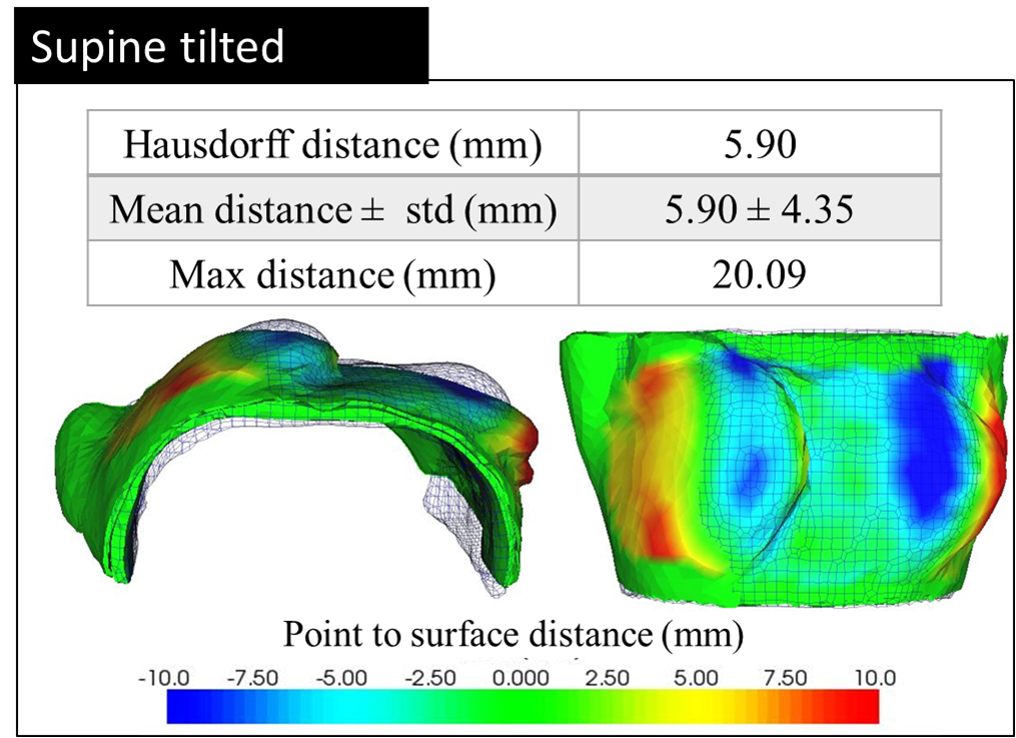
\includegraphics[width=0.9\textwidth,keepaspectratio]{figures/modelevaluation.png} 
\caption{Three breast configurations: prone, supine and supine tilted. First line - MR images in 3 breast configurations. Second and third lines - point to node distance from simulated breast shape (surface mesh) to the measured one (black grid lines).}\label{fig:modelevaluation}
\end{figure}

One may see that the estimated supine tilted breast configuration describes inadequately the breast geometry given by the MR images (Hausdorff distance equal to 5.90 mm). Large difference between simulated and measured breast surfaces is caused by the excessive sliding of breast tissues over the chest wall. Numerical or structural modeling choices could explain such behavior.

Firstly, the fascial and ligamentous tissues are usually characterized by a cable-like behavior. The strain-energy density function must behave asymptotically in order to limit the fascia stretch and thus to reduce non-linearly the breast sliding over the chest wall. Limitations of the neo-Hookean model to capture the mechanical response of some nonlinear materials is well known \citep{kaliske_finite_1997}. For large strain rates, the Neo-Hookean material may undergo a relaxation and therefore becomes easier to deform.  Our experimental results have shown that the maximal strain at the fascia level is significantly higher in supine tilted position (about 140\%) than in supine or prone positions (about 50\%).  Therefore, an asymptotic behavior of fascia mechanical response must be considered.  The Gent  form of strain-energy function characterizes better such mechanical response \citep{gent_new_1996} and should be considered as an alternative choice .

Secondly, the breast support matrix is composed of 4 suspensory ligaments, however only three of them were partially modeled: inframammary, deep medial and deep lateral ligaments. The 3D structures connecting the skin to some muscular areas were neglected, and namely the cranial ligament.  The particularity  of the cranial ligament consist in it's position, almost it's entire structure underlay the skin and the only attachments to the thorax are situated at the clavicle and seventh rib level (inframammary ligament). Including such structures at the skin surface may result in local high strain gradient rates causing solution instability and anesthetic surface deformations. 


\section{Discussions and conclusion} \label{section:validation:discutionconclusion}

In the current part of the manuscript, a new finite elements breast model was proposed and  evaluated with real tissues deformations measured on MR images. To this end, MR images of two patients were acquired in three different configurations: supine, prone and supine tilted. The supine and prone MRI volumes were used to adapt the biomechanical model to the patient individual breast geometry and it's respective tissues mechanical properties.  The optimal mechanical properties were found by exhaustive search over a predefined parameters domain. For each combination of tissues elastic properties,  the breast reference configuration was computed using an adapted prediction-correction iterative scheme. The parameters set giving the best fit between estimated and measured breast configurations were selected.  Using these optimal estimates the supine, prone and supine tilted breast configurations were computed and compared to the MRI volumes.

We found that, extremely soft materials low (0.2-0.3kPa for breast tissues and 4kPa for skin) have to by used in order to obtain the same tissues displacements rate as measured on MR images. Moreover, the breast tissues sliding have to be considered then computing such large deformations. However, because of tissues hyper-elasticity, the model boundary conditions have to be revisited in order to ensure the convergence capability of the solution. With such soft tissues, the finite elements mesh may become highly distorted, then to limit elements distortion a stiffer layer was added between the breast tissues and muscle representing the deep layer of the superficial fascia. The excessive  sliding was prevented by using ligamentous structures fixing the soft tissues on the pectoral muscle.

Contrarely to the previous works, our model is evaluated in 3 breast configurations. Among the 3 geometries, two of them were used for the model optimization and evaluation, and the last one (supine tilted geometry) was used for the evaluation only. Good estimates were obtained in prone and supine configurations with a Hausdorff distance equal to $2.17 mm$ and $1.72 mm$ respectively.  The estimate of the supine tilted breast geometry pointed out the limitations of the Neo-Hookean model to assess rich mechanical behavior of breast soft tissues for large strains. These limitations were not identified in the previous works. 

The model optimization if a tough and time consuming process. It was extremely difficult to obtain the solutions convergence when combining the tissues large deformation with the sliding contact conditions. Because of the lake of time, the reference breast configuration and the optimal constitutive parameters were computed only for the first subject. The model optimization of the second subject is considered for feature work.

Next, we assume that our model describe wall the breast mechanical behavior and  is used to compute breast tissues deformation under compression. The internal tissues strain and the pressure distribution over the skin surface will be used to quantify the patient comfort during the mammography exam. 